\chapter{Implementation}\label{ch:implementation}\glsresetall
Based on \autoref{ch:projectspec}, \nameref{ch:projectspec}, a number of tasks has been set. This chapter clarifies the work done and solutions found to complete the tasks.

\section{YOLO Object Detection}

\section{YOLOv3 Tensorflow Implementation}
As the solution is supposed to work real time, \gls{yolo} was chosen as the desired solution, but also because the CTO had had \gls{yolo} running before using the standard setup of the Darknet running in C trained on the COCO dataset.

Because of the desire to have it running on Tensorflow another version of Darknet is needed, as Tensorflow works with Python and not C. 
Given previous experience with Keras, a solution build upon this is preferred as this will ease the understanding of the implementation and make potential changes to the network easier to do.

\subsection{Keras YOLO3}\label{sec:kerasyolo}
The Keras implementation is found on Github and is made for \gls{yolo}v3. It is based on another repository made with the \gls{yolo}v2 Darknet version, which is a smaller network, but also with a general lower precision \citep{Redmon2016, Redmon2018}. The repository is found at: \url{https://github.com/qqwweee/keras-yolo3}.

This is a conversion of the network design to a Keras implementation. It employs the same annotation layout as the Pascal VOC dataset, which is one row for each image in a text file with every bounding box in the image separated with spaces:

Row format: \lstinline{image_file_path box1 box2 ... boxN}, and box format: \lstinline{x_min,y_min,x_max,y_max,class_id}.

\subsection{Dataset}
It was requested, that the object detection was trained to recognise some industrial objects such as screws, electric fuses for a fuse box and extensions boxes. The dataset chosen is "T-LESS: An RGB-D Dataset for 6D Pose Estimation of Texture-less Objects" made by \cite{tless}. 

As stated in the title of the article for the dataset, the dataset is a an \gls{rgbd} dataset. As \gls{yolo} only works with one type of images only the RGB images are used.

\subsection{Training}
The training is done by running a Python script with Tensorflow which launches the training. Before training, the data needs to be prepared, as the annotation of the dataset differs from the on the network uses.
\subsubsection{Data Preparation}
As the annotations from the T-Less dataset is written in an XML file format with a file for each image of each object, a conversion is necessary. This is done with a small Python script converting to the VOC annotation style mentioned in \autoref{sec:kerasyolo}. The script is found in the appendix. \todo{Indsæt Python script i appendix og henvis rigtigt.}

\subsubsection{Training Setup}
The setup of the network is including a \lstinline{ReduceLROnPlateau} function, which reduces the learning rate when a metric has stopped improving. Another callback function included is \lstinline{EarlyStopping} which stops the training when a certain set improvement is not met for a specified amount of iterations.

\gls{yolo}v3 uses the Darknet-53 \gls{cnn} which has 53 convolutional layers. This is also shown in \autoref{fig:darknet53}. The last \gls{fc} layer has been changed from 1000 classes to 30, as this is the amount of classes included in the T-Less dataset.

\begin{figure}[H]
	\centering
	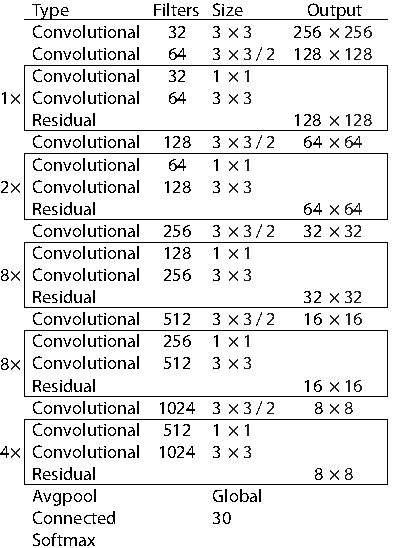
\includegraphics[width=0.45\textwidth]{figures/darknet53}
	\caption{Overview of Darknet-53, the \gls{cnn} used with \gls{yolo}v3 \citep{Redmon2018}}
	\label{fig:darknet53}
\end{figure}

For training the optimiser Adam is used, first with a learning rate of $ 10^{-3} $ if more training is needed after 50 epochs and the learning rate has not been lowered, it is lowered to $ 10^{-4} $, and with a batch size of 32. 

\subsection{Results}\todo{Find resultater på laptop.}


\section{Matrix Storage}
This task was intended as an on stream process, storing the video data before compressing as matrices to a file, to automate testing of the camera compression algorithm. At the point of development, the core solution of the pipeline was written in C++ and not the final GStreamer solution implemented for the video streaming solution.

This task required some insight into the meta solution for pipeline already written and understanding of the code. The code had several dependencies and required some extra in order to generate the data as wanted.

Before reaching a solution to the task, another solution for the pipeline was made and therefore made the task obsolete.

\section{GStreamer Pipeline Configuration}\label{sec:gstream_design}
The pipeline configuration consists of several smaller tasks within the same \gls{gstapp}. In total it has three functions:

\begin{itemize}
	\item Receive RTP packages and store them in desired destination
	\item Receive RTP packages, decompress, and play them back to the user
	\item Decompress the video data and play it for the user
\end{itemize}

The source for the RTP packages is a UDP source, which means an IP and a port needs to be set to receive the packages. When testing, the IP is localhost i.e. \lstinline|127.0.0.1|, and the port depends of which video stream the user wants to receive, as there are both an id stream, a depth video stream and a colour video stream. These are either \lstinline|9000|, \lstinline|9001|, or \lstinline|9002|. It is important to set the same ports on the sender side.

The data received is payloaded and has some h265 encoding which needs depayloading and decoding beofre storing to file or playing back. 

When differing between storing and streaming to a video player, it is only one command in difference. It is either \lstinline|filesink| and a path to destination for storing or \lstinline|fpsdisplaysink| to play back the video.

Besides these settings, it is important to match \textit{caps} which are video settings set from the sender side, and must also be et on the receiver side. These depend on the file type. An example of a GStreamer command to receive and store a video file is:

\noindent\textbf{\lstinline|gst-launch-1.0 videotestsrc num-buffers=100 ! x265enc tune=zerolatency ! video/x-h265, stream-format=byte-stream,alignment=au ! filesink location=h265.pay|}

\section{Docker Set Up}
The docker set up was to be able to test the \gls{gstapp} described in \autoref{sec:gstream_design} having it running in a docker container on an Nvidia TX2.

